\documentclass[a4paper,12pt]{article}
\usepackage[papersize={8.5in,11in},left=2.64cm,right=2.64cm,top=2.64cm,bottom=2.64cm]{geometry}

\usepackage{placeins}
\usepackage{natbib}
\usepackage{lineno}
\usepackage{soul}
\usepackage{url}
\usepackage[colorlinks = true,
            linkcolor = blue,
            urlcolor  = blue,
            citecolor = blue,
            anchorcolor = blue]{hyperref}
            
\linenumbers
%\usepackage[printfigures]{figcaps}

\usepackage[colorinlistoftodos,prependcaption,textsize=tiny]{todonotes}
\usepackage{authblk}
\usepackage{setspace}
\doublespacing
\usepackage{inputenc}

\usepackage{lscape}

%\usepackage[paper=portrait,pagesize]{typearea}


\usepackage{booktabs}
\usepackage{dcolumn}

%\def\settablenum#1{\let\caption\savecaption
%\def\@captype{table}
%\def\thetable{#1} \let\@currentlabel\thetable  \let\label\savelabel}


%opening
\title{Supplementary materials for "The imbricated foreshock and aftershock activities of the Balsorano (Italy) M$_w$ 4.4 normal fault earthquake and implications for earthquake initiation"}


\author{H. S. S\'anchez-Reyes$^1$, D. Essing$^1$, E. Beauc\'e$^2$, P. Poli$^1$}

\affil[1]{Institute of Earth Sciences, University Grenoble Alpes, Grenoble \emph{38100}, France}
\affil[2]{Department of Earth, Atmospheric, and Planetary Sciences, Massachusetts Institute of Technology, Cambridge, MA, United States}
\affil[*]{Corresponding author: hugo.sanchez-reyes@univ-grenoble-alpes.fr}

\date{}                     %% if you don't need date to appear
\setcounter{Maxaffil}{0}
\renewcommand\Affilfont{\itshape\small}



\begin{document}


\maketitle

%% ------------------------------------------------------------------------ %%
%
%  TEXT
%
%% ------------------------------------------------------------------------ %%

\noindent\textbf{Contents of this file}
\begin{enumerate}
 \item Tables S1 to S4 
 \item Figures S1 to S2 
\end{enumerate}

\noindent\textbf{Additional Supporting Information}
\begin{enumerate}
  \item Seismic catalog for the seismic sequence associated to the 2019 (M$_W$ 4.4) Balsorano earthquake
\end{enumerate}




\begin{table}
\renewcommand{\thetable}{S\arabic{table}}
 \caption{General information of the 2019 M$_w$ 4.4 Balsorano earthquake. All this information is taken from the INGV's online catalog.}
 \begin{center}
 \begin{tabular}{@{}l l }
   \hline
    {\hskip 2cm Mainshock data}      &            \\
    \hline
    Magnitude				        & M$_w$ 4.4    \\
    Lat (º) / Lon (º)            	& 13.61 / 41.78  \\
    Depth (km)                      & 14.0           \\    
    NP1: \ Strike / Dip / Rake  	& 299 /	58 / -120   \\
    NP2: \ Strike / Dip / Rake     	& 166 / 42 / -51    \\
    Reported activity 			    & $\approx$ 150 events  \\
   \# Stations $<$ 100 km		    & 6         
 \end{tabular}
 \end{center}
\label{tab:general_info}
\end{table}


\begin{table}
\renewcommand{\thetable}{S\arabic{table}}
\caption{Receiver locations. The distances reported are measured with respect to the mainshock epicentral location (taken from the INGV).}
\begin{center}
 \begin{tabular}{@{} l c c c}
   \hline
    Receiver  & Lon. ($^o$) & Lat. ($^o$) & Dist. (km) \\
    \hline
 CERT & 41.94903 & 12.98176 & 72.297 \\
 GUAR & 41.79450 & 13.31229 & 33.093 \\
 INTR & 42.01154 & 13.90460 & 41.820 \\    
 POFI & 41.71743 & 13.71202 & 13.112 \\
 PTQR & 42.02193 & 13.40057 & 35.780 \\
 VVLD & 41.86965 & 13.62324 & 10.411
 \end{tabular}
\end{center}
\label{tab:general_info}
\end{table}


\begin{table}
\renewcommand{\thetable}{S\arabic{table}}
 \caption{Velocity model used for the relocation process. A V$_P$/V$_S$ ratio equal to 1.73 is assumed. Slightly modified version from the model proposed by \cite{Bagh_2007_BSC}}
 \begin{center}
 \begin{tabular}{@{} c | c}
    \hline
    Depth of top of layer (km)	& P-wave velocity (km/s)  \\
    \hline
    0.0 & 5.360 \\
    3.0 & 5.360 \\
    6.0 & 5.800 \\
    14.0 & 6.650 \\
    25.0 & 6.900 
    \end{tabular}
 \label{tab:velocitymodel}
\end{center}
\end{table}

\begin{landscape}

\begin{table}[!h]
\renewcommand{\thetable}{S\arabic{table}}
 \caption{Reference templates and phase traveltimes at the six available stations (estimated from INGV data).}
 \begin{center}
 \begin{tabular}{@{} l l c c c c c c c c c c c c}
    \hline
      & & P$_{tt}$ & P$_{tt}$ & P$_{tt}$ & P$_{tt}$ & P$_{tt}$ & P$_{tt}$ & S$_{tt}$ & S$_{tt}$ & S$_{tt}$ & S$_{tt}$ & S$_{tt}$ & S$_{tt}$   \\
      \# & Origin time     & CERT & GUAR & INTR & POFI & PTQR & VVLD & CERT & GUAR & INTR & POFI & PTQR & VVLD \\
    \hline
1 & 11/07/2019 00:37:18 & 9.63 & 5.51 & 6.9 & 3.46 & 6.37 & 3.48 & 17.09 & 9.11 & 11.95 & 5.82 & 11.28 & 5.71 \\
2 & 11/07/2019 03:21:00 & 9.72 & 5.38 & 6.92 & 3.57 & 6.62 & 3.57 & 17.15 & 9.4 & 12.12 & 5.87 & 11.36 & 5.82 \\
3 & 11/07/2019 10:37:05 & 9.69 & 5.39 & 6.93 & 3.7 & 6.52 & 3.54 & 17.15 & 9.15 & 12.05 & 6.00 & 11.38 & 5.82 \\
{4} & {11/07/2019 17:35:21} & {9.7} & {5.38} & {7.01} & {3.54} & {6.48} & {3.59} & {17.22} & {9.02} & {12.12} & {5.89} & {11.52} & {5.92} \\
5 & 11/07/2019 17:47:53 & 9.77 & 5.4 & 6.93 & 3.32 & 6.53 & 3.55 & 17.29 & 9.12 & 12.07 & 5.45 & 11.42 & 5.68 \\
6 & 11/07/2019 18:04:55 & 9.74 & 5.35 & 6.9 & 3.39 & 6.54 & 3.49 & 17.21 & 9.12 & 11.86 & 5.68 & 11.45 & 5.72 \\
7 & 11/07/2019 23:19:50 & 9.62 & 5.29 & 7.09 & 3.54 & 6.44 & 3.55 & 16.89 & 8.99 & 12.19 & 6.00 & 11.20 & 5.79 \\
8 & 11/08/2019 03:08:06 & 9.06 & 5.14 & 7.06 & 3.56 & 6.45 & 3.42 & 16.85 & 8.76 & 12.21 & 5.85 & 11.08 & 5.58 \\
9 & 11/08/2019 08:10:56 & 9.93 & 5.56 & 6.75 & 3.17 & 6.72 & 3.37 & 17.33 & 9.23 & 11.69 & 5.39 & 11.58 & 5.48 \\
10 & 11/08/2019 08:16:10 & 9.84 & 5.44 & 6.88 & 3.44 & 6.51 & 3.54 & 17.40 & 9.49 & 12.00 & 5.76 & 11.53 & 5.71 \\
11 & 11/08/2019 10:43:24 & 9.50 & 5.15 & 6.89 & 3.32 & 6.29 & 3.38 & 17.00 & 8.91 & 12.08 & 5.78 & 11.19 & 5.61 \\
12 & 11/08/2019 12:00:43 & 9.75 & 5.44 & 7.04 & 3.34 & 6.61 & 3.55 & 17.29 & 9.13 & 12.44 & 5.70 & 11.35 & 5.77 \\
13 & 11/08/2019 13:07:07 & 9.41 & 5.08 & 6.86 & 3.32 & 6.22 & 3.34 & 16.88 & 8.77 & 12.31 & 5.64 & 11.04 & 5.45 \\
14 & 11/08/2019 14:22:12 & 9.52 & 5.14 & 6.92 & 3.39 & 6.48 & 3.38 & 16.99 & 8.79 & 12.39 & 5.69 & 11.19 & 5.56 \\
15 & 11/09/2019 10:57:09 & 9.72 & 5.35 & 6.87 & 3.21 & 6.54 & 3.46 & 17.20 & 9.03 & 11.98 & 5.52 & 11.33 & 5.70 \\
16 & 11/09/2019 22:14:15 & 9.59 & 5.27 & 6.66 & 3.24 & 6.43 & 3.14 & 17.07 & 9.04 & 11.61 & 5.33 & 10.91 & 5.04 \\
17 & 11/09/2019 23:09:52 & 9.79 & 5.49 & 6.90 & 3.62 & 6.61 & 3.59 & 17.48 & 9.12 & 11.88 & 5.69 & 11.66 & 5.91 \\
18 & 11/10/2019 03:31:36 & 9.55 & 5.15 & 6.58 & 3.51 & 6.37 & 3.42 & 16.82 & 8.68 & 12.21 & 5.79 & 11.07 & 5.55 \\
19 & 11/10/2019 06:56:28 & 9.62 & 5.15 & 6.56 & 3.15 & 6.40 & 3.07 & 17.04 & 9.04 & 11.92 & 5.42 & 11.39 & 5.09 \\
20 & 11/11/2019 01:43:21 & 9.59 & 5.31 & 6.90 & 3.44 & 6.42 & 3.53 & 18.00 & 9.27 & 12.05 & 5.25 & 11.44 & 5.76 \\
21 & 11/11/2019 13:41:33 & 9.46 & 5.11 & 7.00 & 3.49 & 6.22 & 3.39 & 16.81 & 8.79 & 12.20 & 5.85 & 11.10 & 5.54 \\
22 & 11/11/2019 16:04:53 & 9.39 & 5.05 & 6.95 & 3.43 & 6.25 & 3.34 & 17.07 & 8.70 & 12.27 & 5.75 & 11.08 & 5.52 \\
23 & 11/11/2019 17:46:53 & 9.61 & 5.22 & 6.86 & 3.32 & 6.40 & 3.43 & 17.05 & 8.97 & 12.44 & 5.22 & 11.23 & 5.62
    \end{tabular}
 \label{tab:velocitymodel}
\end{center}
\end{table}

\end{landscape}




\begin{figure}
\renewcommand{\thefigure}{S\arabic{figure}}
\begin{center}
 \noindent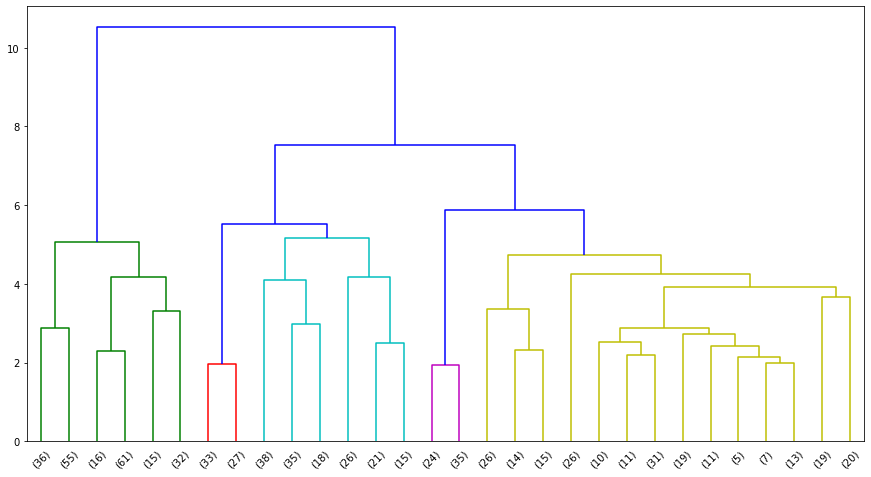
\includegraphics[width=1\linewidth]{dendrogram_balsorano.png} 
\end{center}
\caption{Dendrogram obtained from the waveform-based hierarchical clustering performed. The distance metric between two different waveforms ($i$ and $j$) is estimated as 1-C$_{ij}$. Ward's minimum variance linkage technique is used. The distance threshold to define the final number of cluster is set to 5.3 (the largest separation observed form dendrogram).}
\label{fig:dendrogram}
\end{figure}

\begin{figure}
\renewcommand{\thefigure}{S\arabic{figure}}
\begin{center}
 \noindent 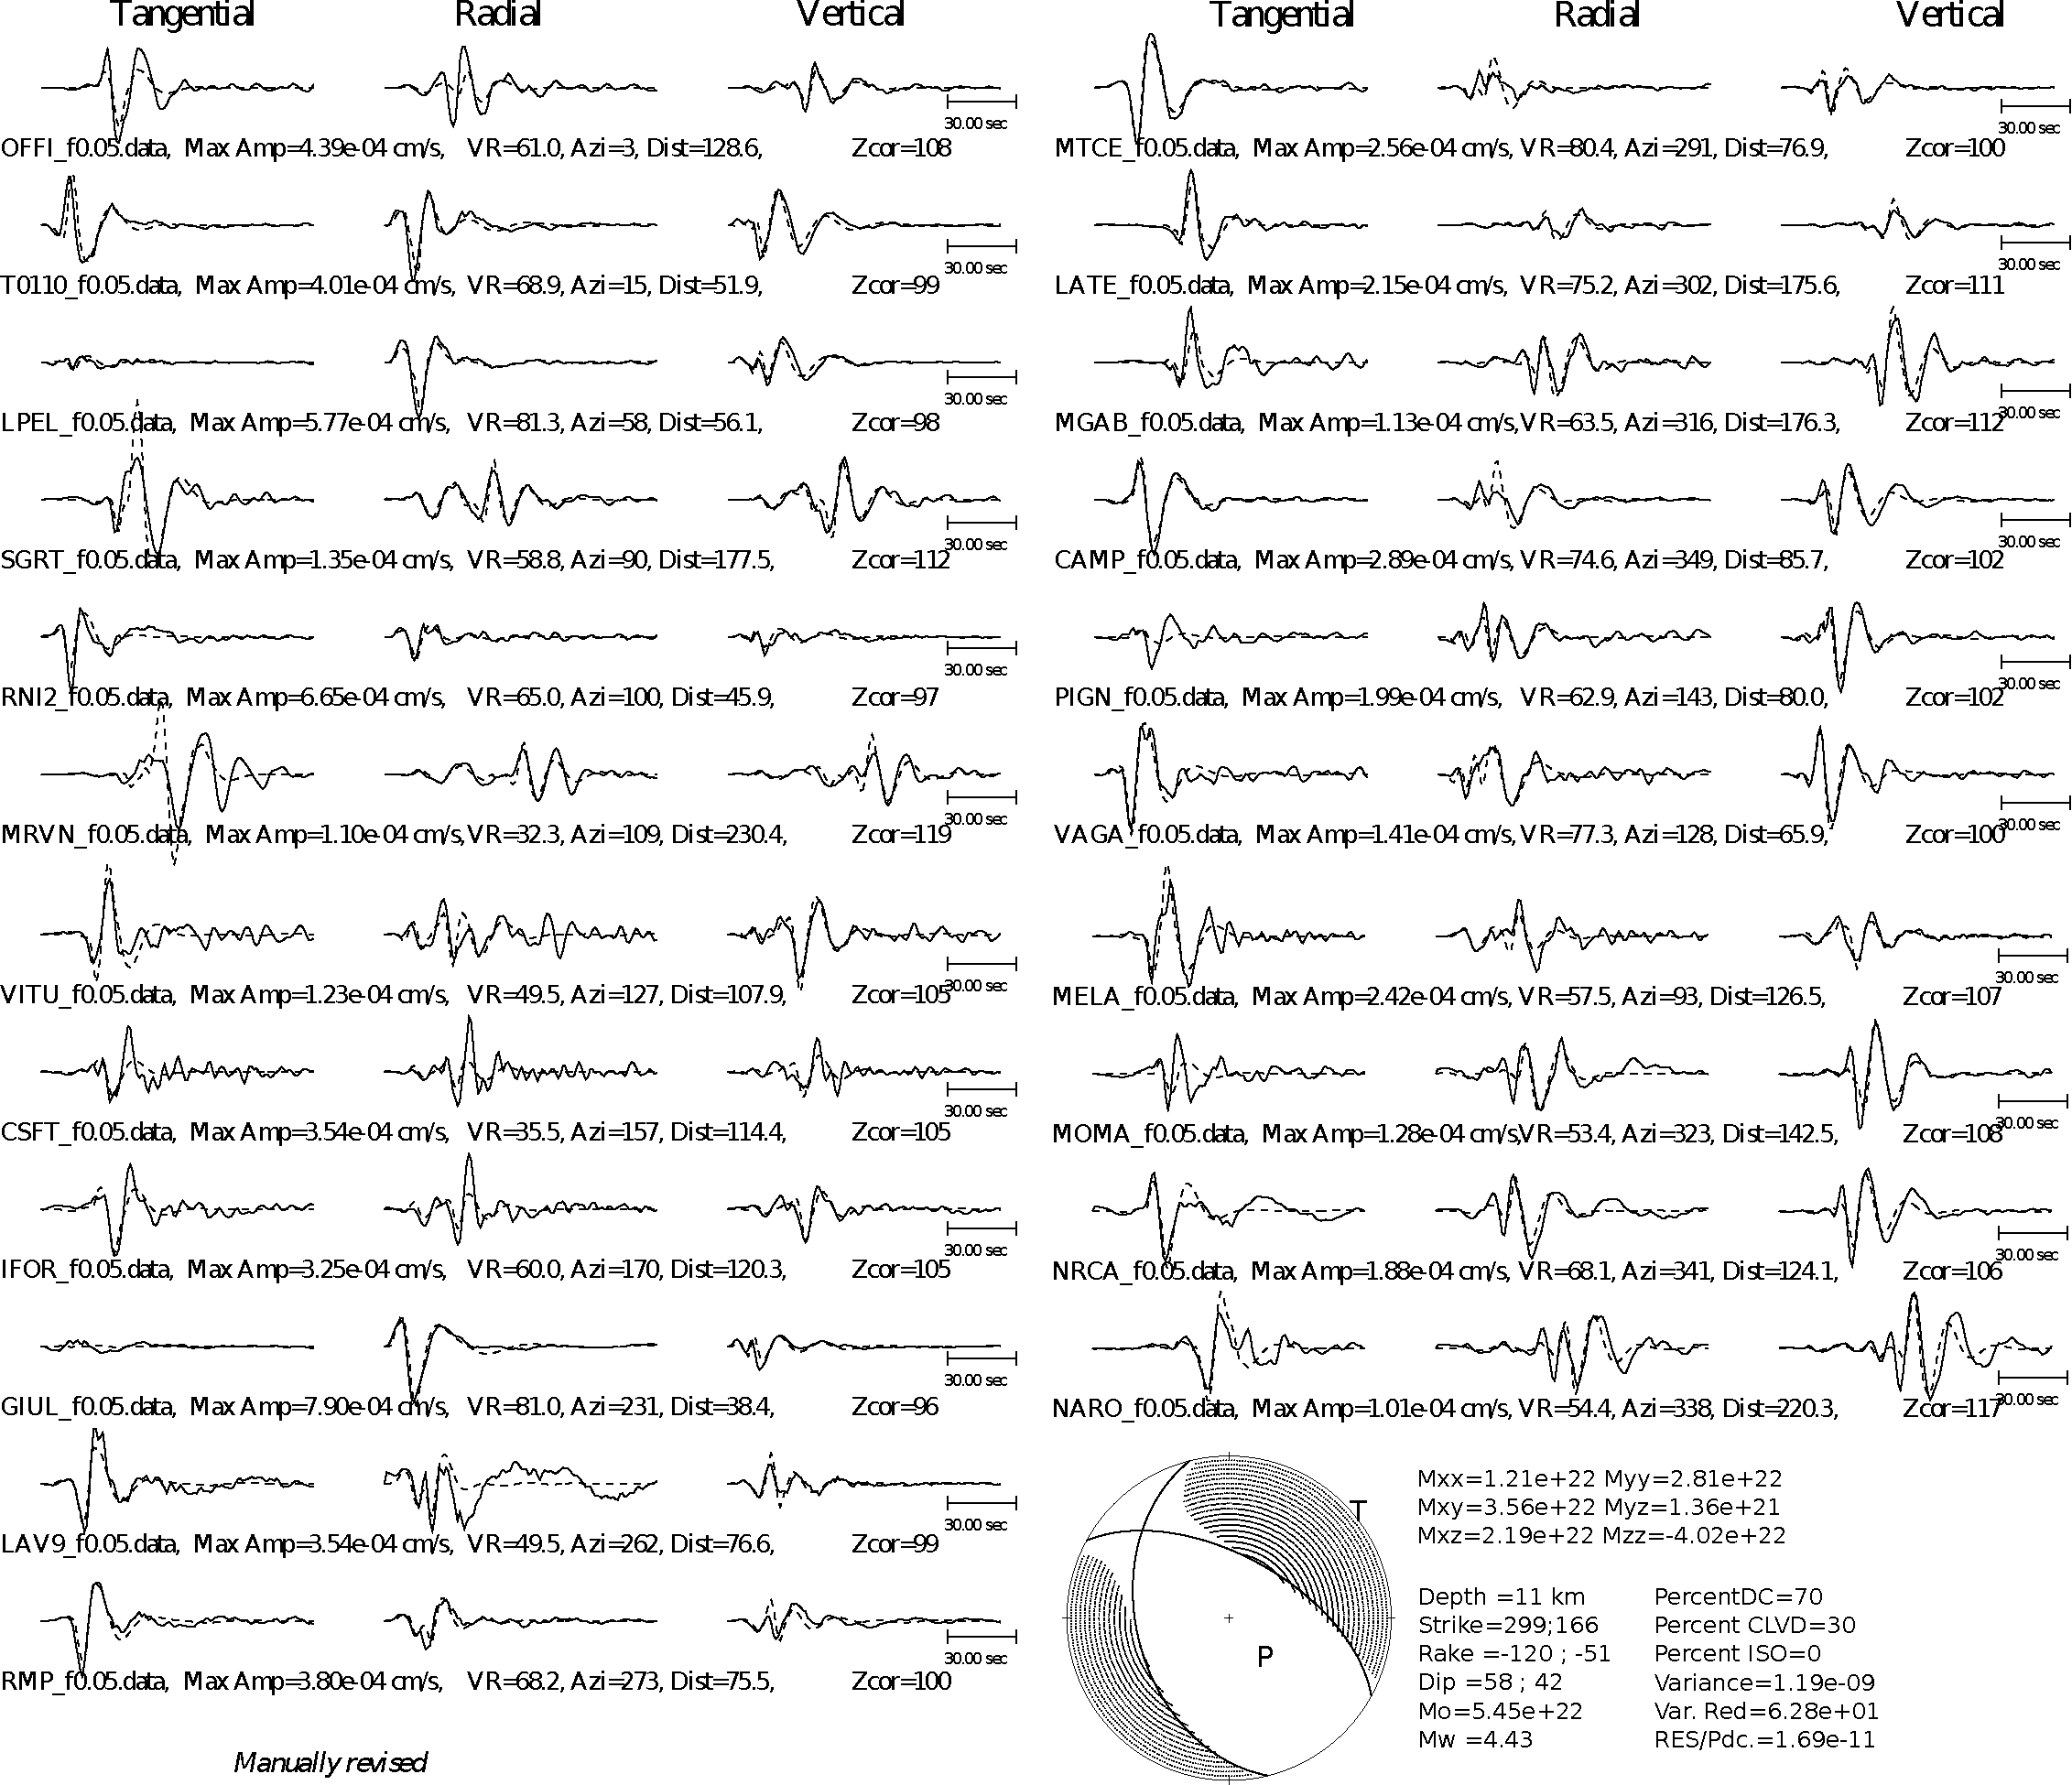
\includegraphics[width=1\linewidth]{S2_Focal_synthetics} 
\end{center}
\caption{Estimated focal mechanism and comparison of observed (solid lines) and estimated synthetic seismograms (dashed lines) for the Mw 4.4 mainshock. The three components at 22 receiver locations are shown. This figure is a modified version from the original one provided by the INGV (\url{http://webservices.ingv.it/webservices/ingv_ws_map/data/tdmt/15111/73711301_86_tdmt_reviewer_solution.pdf}).}\label{fig:S2_focal_mechanism}
\end{figure}


\FloatBarrier

\begin{thebibliography}{}

\bibitem[Bagh et~al., 2007]{Bagh_2007_BSC}
Bagh, S., Chiaraluce, L., De~Gori, P., Moretti, M., Govoni, A., Chiarabba, C.,
  Di~Bartolomeo, P., and Romanelli, M. (2007).
\newblock Background seismicity in the central apennines of italy: The abruzzo
  region case study.
\newblock {\em Tectonophysics}, 444(1-4):80--92.

\end{thebibliography}{}


\end{document}
